\'Etant donn\'e un graphe $G_C = (V_C,E_C)$, l'algorithme suivant a pour but de d\'eterminer la line-couverture si elle existe (notamment si la matrice de corr\'elation est sans erreur). 
Dans le cas contraire, l'algorithme couvrira autant que possible des sommets de $G_C$ par une ou deux cliques.
\newline
Consid\'erons {\cal C} un ensemble de cliques de $G_C$ initialement vide et chaque sommet $v \in V_C$ a un \`etat  $Cliq(v)$ initialis\'e \`a $0$.
\newline
Chaque sommet $v$ a cinq \'etats possibles:
\begin{itemize}
	\item $0$ : il n'est couvert par aucune clique. Il correspond aussi \`a l'\'etat initial des sommets.
	\item $1$ : le sommet $v$ est couvert par une clique ou deux cliques. Dans le cas ou il est couvert par deux cliques, l'intersection de ces cliques donne le sommet $v$.
	\item $2$ : le sommet est couvert par une clique et peut \^etre couvert par une seconde clique.
	\item $3$ : le sommet $v$ est un sommet ambigu.
	\item $-1$ :  le sommet $v$ est couvert par plus de deux cliques. Il doit \^etre corrig\'e par l'algorithme de correction.
\end{itemize}
Pour tout sommet $v$ de degr\'e minimum tel qu'il n'appartient \`a aucune clique ou qu'il est un sommet ambigu, S'il existe une partition coh\'erente de ce sommet et son voisinage $\{v\} \cup \Gamma_G(v)$ en deux cliques $C_1, C_2$, alors ces deux cliques sont contenues dans la line-couverture. Les sommets $v$ et $u$ (avec $u \neq v$), appartenant \`a $C_1$ ou $C_2$, a son \'etat modifi\'e de tel sorte que:
\begin{itemize}
\item $Cliq(v) = 1$ si son \'etat pr\'ec\'edent est \'egal \`a $0$ et la clique $C_2$ est vide. 
\item $Cliq(v) = 3$ si son \'etat pr\'ec\'edent est \'egal \`a $0$ et la clique $C_2$ est non vide. 
\item $Cliq(v) = 2$ si son \'etat pr\'ec\'edent est diff\'erent de $0$.
\item $Cliq(u) = 1$ si son \'etat pr\'ec\'edent est \'egal \`a $0$ et l'ensemble des ar\^etes incidentes \`a $u$ est vide.
\item $Cliq(u) = 2$ si son \'etat pr\'ec\'edent est \'egal \`a $3$ et l'ensemble des ar\^etes incidentes \`a $u$ est vide.
\item $Cliq(u) = 3$ si son \'etat pr\'ec\'edent est \'egal \`a $0$ et l'ensemble des ar\^etes incidentes \`a $u$ est non vide.
\item $Cliq(u) = -1$ si son \'etat pr\'ec\'edent est \'egal \`a $3$ et l'ensemble des ar\^etes incidentes \`a $u$ est non vide.
\end{itemize} 
Dans le cas ou il n'existe aucune partition coh\'erente au sommet $v$, son \'etat est \`a $Cliq(v)=-1$.

\begin{algorithm}
\caption{couverture\_cliques}
\noindent DEBUT\\
\noindent 1. {\bf Si} $G$ est isomorphe \`a un graphe double (voir figure \ref{graphe2Couverture} ), {\bf alors} le traiter avec Verif\_correl$(^1)$ \\
~~\indent {\bf Sinon} \\
~2. \indent {\bf Tant que} il existe un sommet $u$ t.q $Cliq(u) \in \{0,3\}$\\ 
       	\indent~~~~~~{\bf Faire}\\
~3.	       	\indent~~~~~~~~choisir $u$ de degr\'e minimum\\
~4.       	\indent~~~~~~~~{\bf Si} $\{u\} \cup \Gamma_G(u)$ peut \^etre couvert par deux cliques $C_1$ et $C_2$ coh\'erentes,\\
		\indent~~~~~~~~~~~~~~$C_1$ maximale et $C_2 = \emptyset$ si $Cliq(u)=3$ $(^2)$\\
	       	\indent~~~~~~~~~~~~{\bf alors}\\
~5.	       	\indent~~~~~~~~~~~~~~{\bf Si } $Cliq(u) = 0$ et $C_2\neq \emptyset$ {\bf Alors} $Cliq = 3$ \\
~6.		\indent~~~~~~~~~~~~~~{\bf Sinon Si} $Cliq = 0$ et $C_2 =  \emptyset$ {\bf Alors} $Cliq(u) = 1$\\
~7.		\indent~~~~~~~~~~~~~~~~~~~~~~~{\bf Sinon} $Cliq(u) = 2$ 	\\
~8.		\indent~~~~~~~~~~~~~~~~~~~~~~~{\bf FinSi}\\      	
~9.		\indent~~~~~~~~~~~~~~{\bf FinSi}\\
~10.		\indent ~~~~~~~~~~~~~$\epsilon_u = E(G[C_1]) \cup E(G[C_2])$\\
~11.		\indent ~~~~~~~~~~~~~{\bf Pour tout} $w \in \Gamma_G(u)$ {\bf Faire} \\
~12.		\indent~~~~~~~~~~~~~~~~$\alpha(w) = card\{[w,x] \in E - \epsilon_u\}$\\
~13.		\indent~~~~~~~~~~~~~~~~{\bf Si} $\alpha_w > 0$ {\bf Alors}\\
~14.		\indent~~~~~~~~~~~~~~~~~~{\bf Si} $Cliq(w) = 0$ {\bf Alors} $Cliq(w) =3$\\
~15.		\indent~~~~~~~~~~~~~~~~~~{\bf Sinon Si} $Cliq(w) = 3$ {\bf Alors} $Cliq(w) =-1$\\
~16.		\indent~~~~~~~~~~~~~~~~~~{\bf FinSi} \\
~17.		\indent~~~~~~~~~~~~~~~~{\bf Sinon Si} $Cliq(w) = 0$ {\bf Alors} $Cliq(w) =1$\\
~18. 	\indent~~~~~~~~~~~~~~~~~~~~~~~~~{\bf Sinon Si} $Cliq(w) = 3$ {\bf Alors} $Cliq(w) = 2$ \\
~19. 	\indent~~~~~~~~~~~~~~~~~~~~~~~~~{\bf FinSi} \\
~20.		\indent ~~~~~~~~~~~~~{\bf FinPourTout}\\
~21.		\indent ~~~~~~~~~~~~~$E = E - \epsilon_u$\\
~22.		\indent            ~~~~~~~{\bf Sinon} $Cliq(u) = -1$\\
	       	\indent~~~~~~~~~~~~{\bf FinSi}\\
%       	\indent~~~~~~
~23. \indent {\bf FinTant que}\\
~24. \noindent {\bf Fin Si}\\
\noindent FIN\\
\end{algorithm}

$^1$ : chaque graphe de la figure \ref{graphe2Couverture} admet deux line-couvertures, souvent isomorphes, mais (au plus) une seule de ces line-couvertures correspond au DAG du r\'eseau \'electrique sous-jacent. Dans ce cas, on utilise les mesures de correlation de la matrice de mesures $\mu_C$ afin de d\'eterminer pla plus probable entre les deux.
\newline

 $^2$ :  le sommet $u$ choisi (s'il existe) ne sera pas prioritairement un sommettel que $Cliq(u) = 0$ et $u$ est un point d'ambiguit\'e. Si lors d'une \'etape, seul un tel choix est possible et qu'il n'y a aucun sommet $u$ tel que $Cliq(u) = -1$, c'est que chaque sommet du graphe initial $G$ est un point d'ambiguit\'e.
 Dans ce cas, $G_C$ est une union de composantes connexes isomorphes \`a un des graphes de la figure  \ref{graphe2Couverture}.
Dans ce cas, n'importe quel choix conduit \`a une d\'ecomposition correcte.
Dans tous les autres cas de sommet choisi $u$, le lemme \ref{lemmaCoherente} montre que le choix de d\'ecomposition est unique si $G$ est un line graphe.
\newline

La partition coh\'erente se d\'etermine au moyen des mesures physiques selon la loi de conservation des noeuds. 
En effet, tous les sommets d'une clique dans un line graphe sont des ar\^etes qui concourent un sommet du r\'eseau \'electrique. 
Par les lois d'\'electricit\'es, la diff\'erente entre les flots entrant et sortant dans ce sommet correspond aux pertes par effets joules $EJ$. 
Ainsi les deux cliques s'obtiennent si cette diff\'erence est inf\'erieure aux pertes joules.
Dans notre algorithme de couverture, nous supposons que la partition coh\'erente propos\'ee est toujours exacte. Cela signifie que nous connaissons la valeur des pertes par effets joules dans le r\'eseau \'electrique. Dans le cas ou ce param\^etre est inconnu, quel est la valeur minimum de ces pertes not\'ee $\epsilon$ \`a partir duquel la partition est toujours exacte?
En d'autres termes, quel est la valeur $\epsilon$ pour laquelle la d\'ecision de l'ORACLE est un {\em vrai positif}, L'ORACLE \'etant la fonction retournant les partitions coh\'erentes. 
La decision de l'ORACLE est la valeur $\epsilon$.

\subsubsection{Impact des pertes par effets joules}
%epsilon est le taux min des pertes par effets joules pour lequel l'oracle ne comet pas d'erreurs.
% EJ ce sont les pertes par effet joules dans le reseau.
Nous consid\'erons que le r\'eseau \'electrique est connu et que sa matrice de corr\'elation est correcte. 
Dans le but d'\'etudier le taux minimum des pertes par effets joules not\'ee $epsilon$ dans le r\'eseau afin que la partition coh\'erente propos\'ee (appel\'ee ORACLE) soit toujours correcte, nous r\'ealisons deux exp\'eriences: 
\begin{itemize}
\item La premi\`ere  exp\'erience consiste \`a fixer la d\'ecision de l'ORACLE $\epsilon=cte$ tout en g\'en\'erant des mesures dans le graphe. Ces mesures subissent les variations des pertes par effets joules de $0$ \`a $1$ par pas de $0.125$ $EJ=[0,1]$. 
Nous etudions l'\'evolution de la distance de Hamming (ou coefficient de similarit\'e) en fonction de pertes joules $EJ$. 
\item La deuxi\`eme exp\'erience consiste \`a faire varier la d\'ecision de l'ORACLE. Nous etudions les variations des pertes en fonctions de la decision de l'ORACLE.  Les pertes par effets joules $EJ$ de $0$ \`a $1$ par pas de $0.125$. 
%\item La premi\`ere  exp\'erience consiste \`a g\'en\'erer des mesures dans le graphe de tel sorte que les pertes par effets joules $EJ$ soient constantes c'est-\`a-dire $EJ = cte$. 
%\item La deuxi\`eme exp\'erience consiste \`a faire varier les pertes par effets joules $EJ$ de $0$ \`a $1$ par pas de $0.1$. 
\end{itemize}
Rappelons que $EJ=0.1$ signifie qu'il existe une diff\'erence de flot par grandeurs entre les arcs ext\'erieures (sortantes) et int\'erieures (entrantes) \`a chaque sommet. Ainsi $EJ=0$ signifiant qu'il n'existe aucune perte tandis que  $EJ=1$ signifiant qu'il n'existe aucuns flots entre les arcs entrants et sortants d'un sommet du r\'eseau de flots.
% experience 1
\paragraph{exp\'erience 1} :
On fixe la d\'ecision de l'ORACLE \`a $\epsilon=0,75$. 
La figure \ref{courbeEJCoef} resume les variations de l'ORACLE. 
Le fait que la courbe de d\'ecision de l'ORACLE est d\'ecroissante conforte notre hypoth\`ese selon laquelle il n'existe aucuns flots entre les arcs entrants et sortants d'un sommet lorsque les pertes par effets joules sont \'egales \`a $1$. En effet, pour toute valeur de pertes par effets joules  $EJ=[0,0.3]$, le graphe propos\'e est identique au graphe du r\'eseau \'electrique. Par contre, l'ORACLE se trompe deux sur trois sur les cliques fournies pour $EJ = ]0.3,0.9]$ parce que la distance de Hamming est de $0.38$. 

%experience 2
\paragraph{exp\'erience 2} :
Ici, on suppose la similarit\'e \'egale \`a 1 et on cherche les variations de l'ORACLE $\epsilon$ en fonction des pertes par \textit{effets joules}. 
Les pertes par \textit{effets joules} varient de $[0,1]$ par pas de $0.125$ et nous distinguons $8$ intervalles [0,0.125], ]0.125,0.250], ]0.250,0.375], ]0.375,0.5], ]0.5,0.625], ]0.625, 0.75], ]0.75,0.875], ]0.875,1]. 
Pour chaque valeur $\epsilon$, on compte les intervalles $EJ_x, x \in [1,8]$ dans lesquelles la distance de Hamming est \'egale \`a $1$ not\'e $X(\epsilon)$. Ainsi $X(\epsilon=0.3) = 8$ signifie que  les pertes par effets joules varient de $0$ \`a $1$ (EJ=[0,1]) et $X(\epsilon=0.3) = 2$ correspond \`a une variation de $EJ$ sur l'intervalle $[0,0.250]$.
On cr\'ee ainsi la distribution des d\'ecisions de l'ORACLE en fonction des pertes par effets joules.
La figure \ref{courbeEpsilonEJ}  r\'esume cette distribution qui varie de $1$ (correspondant \`a une variation sur [0,0.125]) \`a $8$ (correspondant \`a une variation sur [0,1]).
la courbe de cette distribution est constante de l'intervalle $\epsilon = [0,0.125]$ puis  d\'ecroissante de l'intervalle $\epsilon =[0.125,1]$ et cette pente est tr\`es accentu\'ee dans l'intervalle $\epsilon = [0.8, 1]$. 
Au d\'el\`a  de $\epsilon > 0.8$, les pertes $EJ$ varient dans l'intervalle $EJ=[0,0.2]$.
On en conclut que le meilleur intervalle est $\epsilon = [0.8, 1]$ pour produire des graphes de distances de Hamming \'egale \`a $1$ en pr\'esence de pertes par \textit{effets joules} de $20\%$.

% images
\begin{figure}
\centering
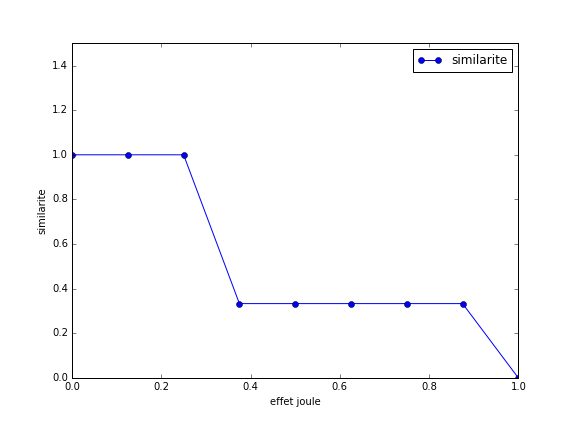
\includegraphics[scale=0.50]{courbe_similarite_selon_EJ_pour_epsilon_075.png}
\caption{ La distance de Hamming en fonction des pertes par \textit{effets joules} pour $epsilon=0.75$ }
\label {courbeEJCoef}
\end{figure}
\begin{figure}
\centering
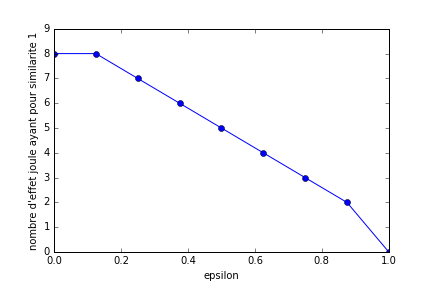
\includegraphics[scale=0.65]{courbe_epsilon_selon_nbreEJ_pour_similarite_1.png}
\caption{ r\'elation inverse entre epsilon et EJ: 8 en ordonn\'e correspond \`a [0,1], 7 \`a [0, 0.875] }
\label {courbeEpsilonEJ}
\end{figure}

% conclusion
Ces deux exp\'eriences montrent que la d\'ecision de l'ORACLE $(\epsilon)$ a une r\'elation inverse avec les pertes par effets joules ($EJ$). En effet, plus epsilon est petit plus les pertes par effets joules sont grandes et plus les decisions de l'ORACLE sont erron\'ees.
\begin{equation}
	\epsilon > 1 - EJ
\end{equation}

\subsubsection{Complexit\'e de l'algorithme de couverture}
La complexit\'e de l'algorithme est au pire en $O(m \times \Delta(G_C))$ avec $m$ le nombre d'ar\^etes et $\Delta(G_C)$ le degr\'e maximum du graphe.
On rappelle que l'algorithme de Lehot \cite{decompositionEnCliques} a une complexit\'e en $O(m)$. 
Le facteur $\Delta(G_C)$ dans notre algorithme, du \`a la recherche de la decomposition en deux cliques $C_1$ et $C_2$ est n\'ecessaire \`a la determination de l'ensemble des sommets $v$ tels que $Cliq(v) = -1$, en nombre le plus petit possible.
\newline

En conclusion, si le graphe $G_C$ est bien un line graphe, l'algorithme trouvera une d\'ecomposition du voisinage d'un sommet en une ou deux cliques de fa\c con unique (voir les lemmes pr\'ec\'edents). 
Une fois ce sommet supprim\'e, le graphe restant est toujours un line graphe, et la propri\'et\'e se propage.
Donc, si $G_C$ est un line graphe, l'algorithme en trouvera toujours la couverture de corr\'elation unique.
